\documentclass[12pt, a4paper]{article}
\usepackage[utf8]{inputenc}
\usepackage[hyphens]{url}
\usepackage{
    amsmath, amssymb, amsfonts, 
    amsthm, lipsum, 
    physics, mathtools, setspace,
    array, caption, float,
    tikz, tikz-3dplot, multicol,
    stackengine, enumitem, subfig
}

\usepackage[hmarginratio=1:1, margin=0.5in, includeheadfoot]{geometry}

\graphicspath{ {./res/} }
\usetikzlibrary{decorations.markings}
\usetikzlibrary{angles, quotes}
\newcommand{\neswarrow}{\ensurestackMath{\stackengine{0pt}{\nearrow}{\swarrow}{O}{c}{F}{F}{L}}}

% \doublespacing 

\usepackage{xcolor}
% \pagecolor[rgb]{0.128,0.128,0.128}
% \color[rgb]{1,1,1}
\title{\vspace{-2cm}Applications of Quaternions in 3D Rotation}
\author{Martin Velikov}
\date{To what extent can quaternions supersede rotation matrices constructed from Euler
    angles in representing 3D rotation?}

\begin{document}
\maketitle
\tableofcontents

\pagebreak

\section{Introduction}
Historically, mathematicians have endeavoured to accurately describe the real
world around us using mathematics. One of the most fundamental necessities of
working with geometry applicable to real life is the ability to reason about
mathematical properties in three dimensions. In the modern day, demand for
working in three dimensions is ever increasing, with scientific applications in
aerodynamic modeling, astrophysics, robotics and computational chemistry, in
addition to numerous uses in computer generated imagery (CGI). In all of these
use cases, there is a need for a rigorous mathematical framework to represent
and manipulate the 3D world. \\

One of the intuitively simplest, but surprisingly complex aspects of
transitioning from a two dimensional space to three dimensional is the problem
of rotation. Indeed, there currently exist several competing mathematical models
for 3D rotation in common use which bear their own strengths and weaknesses. Of
these, some of the most common are 3D ``rotation matrices'' (which are usually
constructed from ``Euler angles"), and ``quaternions'' (Huynh, 2009).\\


This investigation aims to explore the extent to which quaternions can perform
better than rotation matrices constructed from Euler angles in representing 3D
rotation, in order to draw conclusions about the applicability and usefulness of
different rotation methods in computer graphics and scientific simulations. \\

As an aspiring computer animator and game developer, this question is of real
significance to me as it will provide invaluable experience in the underlying
concepts of my field of work for me. The understanding of rotation methods I
would gain from this essay will allow me to apply mathematical knowledge to game
prototypes I create, especially when programming physics or movement systems.
Additionally, from online forums, I have noticed that developers working on the
creative part of their work often do not understand mathematical concepts
underpinning tools they work with daily, and this leads to ambiguity and
confusion when communicating with other developers, or while working. Often, I
feel like this could be due to the exaggerated barrier of entry to learning the
underlying mathematics, leaving many afraid to investigate in the first place. I
hope that this work will help me and others in demistyfing how quaternions and
rotation matrices work, in addition to showing why and when they are useful in
an accessible manner. In order to build intuition for myself and the reader,
nearly all of the formulas and proofs in this essay are of my own independent
derivation, with some external sources used for inspiration and guidance, which
should hopefully demonstrate that one does not need a tertiary education degree
to investigate this topic holistically, and I find this very important to making
mathematics accessible to everyone. \\

In order to answer the question, I first build intution for the reader by
examining how rotation works in two dimensions by introducing the concept of
rotating axes using two dimensional transformation matrices, and then extend
this to the three dimensions. I then introduce and evaluate the concept of Euler
angles and link them with how they can be used to construct 3D rotation
matrices. Following this, I introduce the concept of quaternions from their
original definition and independently develop fundemental rules for operations
with them. Finally, I investigate how quaternions can be used to represent 3D
rotation and compare various aspects of their performance to rotation matrices
constructed from Euler angles in order to draw conclusions about whether one
could supersede the other in representing 3D rotation.

\pagebreak

\section{Rotation Matrices}
Rotation matrices are considered one of the most versatile and fundamental ways
of doing 3D rotation. They are often used in computer animation and praised for
their computational efficiency and versatility. Mathematically, they represent a
3D linear transformation which, when applied to a set of points, describes a 3D
rotation.

\subsection{In two dimensions}
It is worthwile conceptually exploring what happens in two dimensions first, as
this will introduce valuable concepts which will help with understanding how
three dimensional rotation matrices work. \\

Let 2D points be represented as a position vector of the form $\vec{v} =
        \begin{bmatrix}x \\ y\end{bmatrix}$ where $x$ and $y$ represent the x
        and y coordinates of the point respective to the origin. \\

By representing the points as vectors, rotation of a point around the origin
would be equrivalent to rotating its position vector. Consider the rotation of
point (1, 0) by 45 degrees anti-clockwise:

\begin{figure}[H]
    \centering
    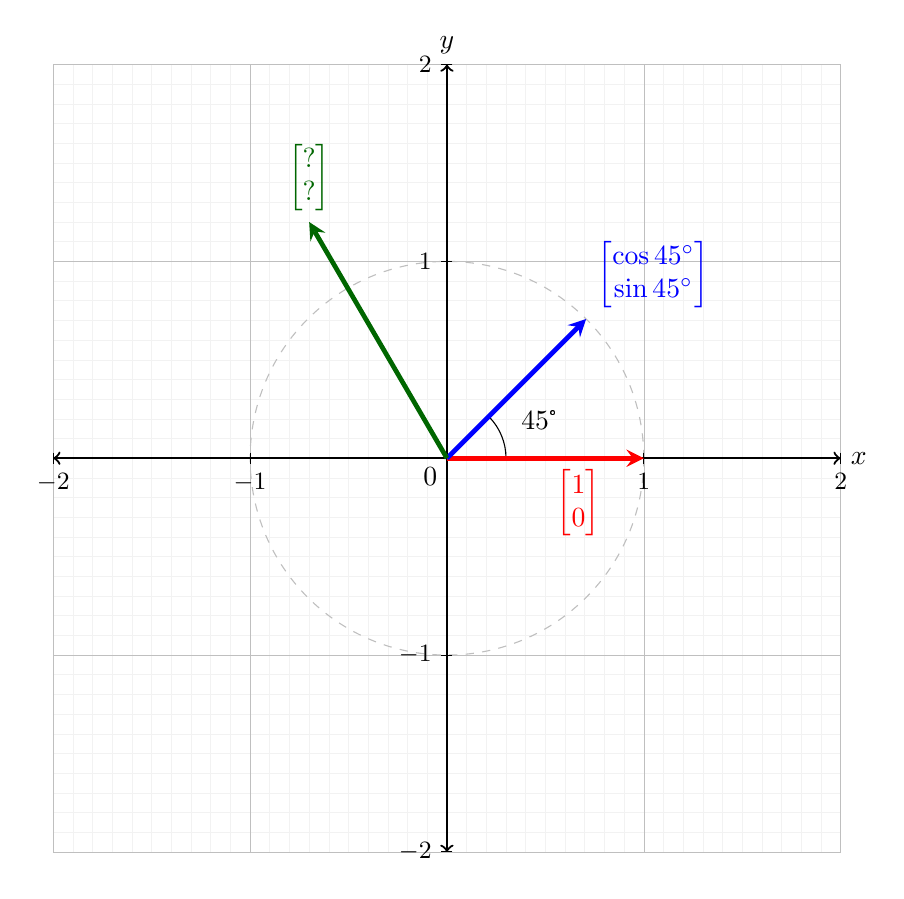
\begin{tikzpicture}[x=2.5cm,y=2.5cm]
        \coordinate (Origin) at (0, 0);
        \coordinate (R) at (0.7071, 0.7071);
        \coordinate (P) at (1, 0);

        % Draw grid
        \draw[gray!10, very thin, step=0.1] (-2, -2) grid (2, 2);
        \draw[gray!50, very thin, step=1] (-2, -2) grid (2, 2);

        \draw[gray!50, dashed] (0, 0) circle (1);

        % Draw tick marks on the axes
        \foreach \x in {-2, -1, 1, 2}
        \draw (\x, 2pt) -- (\x, -2pt) node[below] {\small $\x$};
        \foreach \y in {-2, -1, 1, 2}
        \draw (2pt, \y) -- (-2pt, \y) node[left] {\small $\y$};

        \node[below left] at (0, 0) {$0$};

        % Draw Cartesian axes
        \draw[<->, thick] (-2, 0) -- (2, 0) node[right] {$x$};
        \draw[<->, thick] (0, -2) -- (0, 2) node[above] {$y$};

        \pic[draw, angle radius=0.75cm, angle eccentricity=1.7, "$45$\textdegree"] {angle=P--Origin--R};

        % Draw red vector arrow [1, 0]
        \draw[->, red, line width=0.6mm, >={stealth}] (0, 0) -- (P) node[midway, below right] {$\begin{bmatrix}1 \\ 0\end{bmatrix}$};

        % Draw blue vector arrow [0.7071, 0.7071]
        \draw[->, blue, line width=0.6mm, >={stealth}] (0, 0) -- (R) node[above right]
            {$\begin{bmatrix}\cos 45^\circ \\ \sin 45^\circ\end{bmatrix}$};

        \draw[->, black!60!green, line width=0.6mm, >={stealth}] (0, 0) -- (-0.7, 1.2) node[above]
            {$\begin{bmatrix}? \\ ?\end{bmatrix}$};

    \end{tikzpicture}
    \caption{ Apparent rotation of red vector $\begin{bmatrix}1 \\ 0\end{bmatrix}$ by
        45\textdegree \space anti-clockwise to form blue vector }
    \label{2d_rot}
\end{figure}

From Figure \ref{2d_rot}, it becomes evident that rotating the red vector of
length $1$ that lies along the $x$ axis around a unit circle by $\theta$ degrees
anti-clockwise is equrivalent to finding a point on the unit circle at angle of
$\theta$ degrees to the horizontal. Hence, for any angle $\theta$, the rotation
of $\begin{bmatrix}1 \\ 0\end{bmatrix}$ is equal to $\begin{bmatrix}\cos\theta
\\
        \sin\theta\end{bmatrix}$. \vspace{0.2cm}

Indeed, this is the case for the simple example of a 2D unit vector above, but
the applicability of using trigonometric functions to individually compose a
vector's components grows increasingly limited as the complexity of the problem
at hand increases. For example, consider the case where one would like to rotate
several thousand, or millions of points by the same angle, as is often the case
in computer graphics. In this case, it would be inefficient (and computationally
expensive) to calculate the sine and cosine of the angle to each point
individually, and this operation would also be equally expensive to reverse for
a large number of points. \\

Linear transformation using matrices elegantly deals with these problems by
introducing one concept - instead of transforming each individual vector, we can
transform the axes themselves. \\

\begin{figure}[H]
    \centering
    \vspace{0.5cm}
    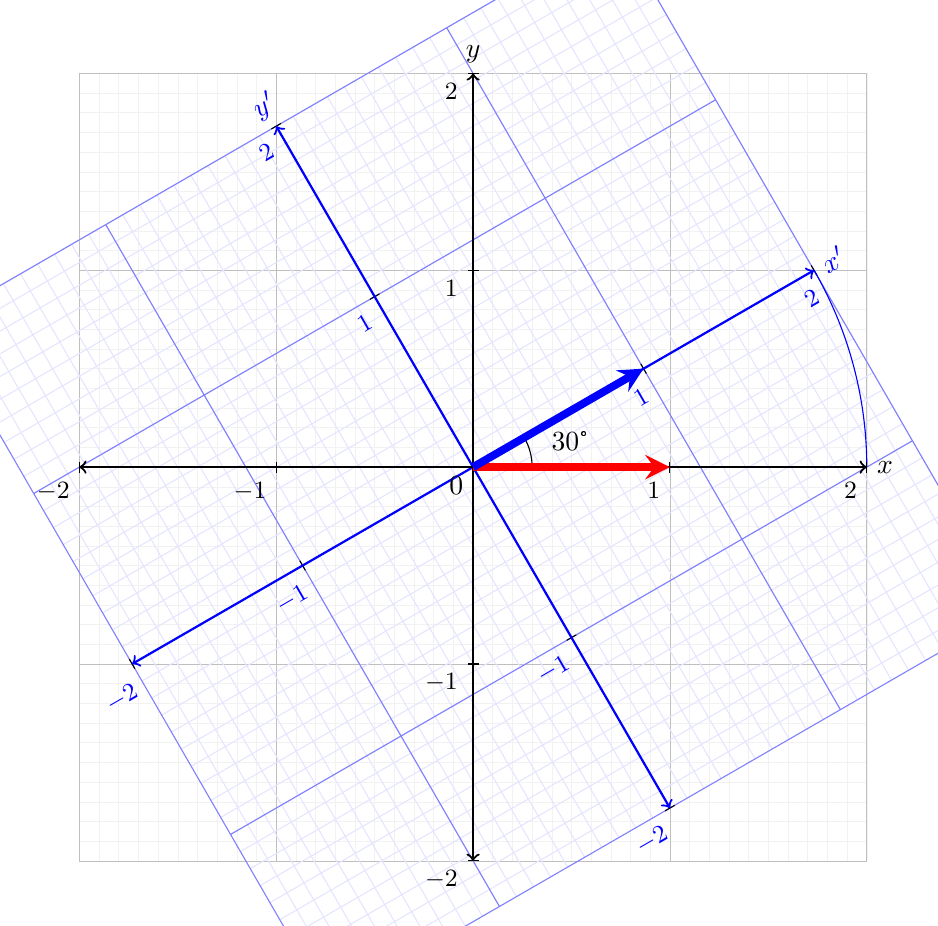
\begin{tikzpicture}[x=2.5cm,y=2.5cm]
        \coordinate (Origin) at (0, 0);
        \coordinate (R) at (0.8660, 0.5);
        \coordinate (P) at (1, 0);

        % Draw grid
        \draw[gray!10, very thin, step=0.1] (-2, -2) grid (2, 2);
        \draw[gray!50, very thin, step=1] (-2, -2) grid (2, 2);

        % 45deg
        \rotatebox{30}{
            \draw[step=0.1, blue!10, very thin, thin] (-2,-2) grid (2,2);
            \draw[step=1, blue!50, very thin, thin] (-2,-2) grid (2,2);

            \foreach \x in {-2, -1, 1, 2}
            \draw (\x, 2pt) -- (\x, -2pt) node[blue, below left] {\small $\x$};
            \foreach \y in {-2, -1, 1, 2}
            \draw (2pt, \y) -- (-2pt, \y) node[blue, below left] {\small $\y$};

            \draw[<->, blue, thick] (-2, 0) -- (2, 0) node[right] {$x'$};
            \draw[<->, blue, thick] (0, -2) -- (0, 2) node[above] {$y'$};
        }

        \pic[draw, blue, angle radius=5cm] {angle=P--Origin--R};

        % Draw tick marks on the axes
        \foreach \x in {-2, -1, 1, 2}
        \draw (\x, 2pt) -- (\x, -2pt) node[below left] {\small $\x$};
        \foreach \y in {-2, -1, 1, 2}
        \draw (2pt, \y) -- (-2pt, \y) node[below left] {\small $\y$};

        \node[below left] at (0, 0) {$0$};

        % Draw Cartesian axes
        \draw[<->, thick] (-2, 0) -- (2, 0) node[right] {$x$};
        \draw[<->, thick] (0, -2) -- (0, 2) node[above] {$y$};

        \pic[draw, angle radius=0.75cm, angle eccentricity=1.7, "$30$\textdegree"] {angle=P--Origin--R};

        % Draw red vector arrow [1, 0]
        \draw[->, red, line width=1mm, >={stealth}] (0, 0) -- (P);

        % Draw blue vector arrow [0.7071, 0.7071]
        \draw[->, blue, line width=1mm, >={stealth}] (0, 0) -- (R);
    \end{tikzpicture}

    \vspace{1.5cm}
    \caption{ Overlay of new cartesian plane (blue) with axes $x'$ and $y'$
        rotated 30\textdegree \space anti-clockwise relative to the original
        axes. }
    \label{2d_axis_rot}
\end{figure}

In Figure \ref{2d_axis_rot}, the blue vector's coordinates on the rotated axes
are identical to the red vector's coordinates on the original axes - both are
$\begin{bmatrix}1 \\ 0\end{bmatrix}$ in their respective axes. In fact, any one
point on the original axis has a counterpart on the rotated axis which
corresponds to the rotation of that point about the origin by $30$\textdegree.
If we examine the coordinates of the blue vector $b$ on the original axes, we
find that
$
    \vec{b}
    =
    \begin{bmatrix}
        \frac{\sqrt{3}}{2}\\ \frac{1}{2}
    \end{bmatrix}
    =
    \begin{bmatrix}
        \cos 30^\circ \\
        \sin 30^\circ
    \end{bmatrix}
$, which aligns with findings from the trigonometric method explored earlier above. \\

In practice, the idea of transforming the axes is integral to the speed of many
3D applications, because linear transformation matrices are not limited to just
rotation. As we will soon find, it is possible to scale, warp and reflect a set
of point vectors with the very same mathematical method, at no extra
computational expense.

\begin{figure}[H]
    \centering
    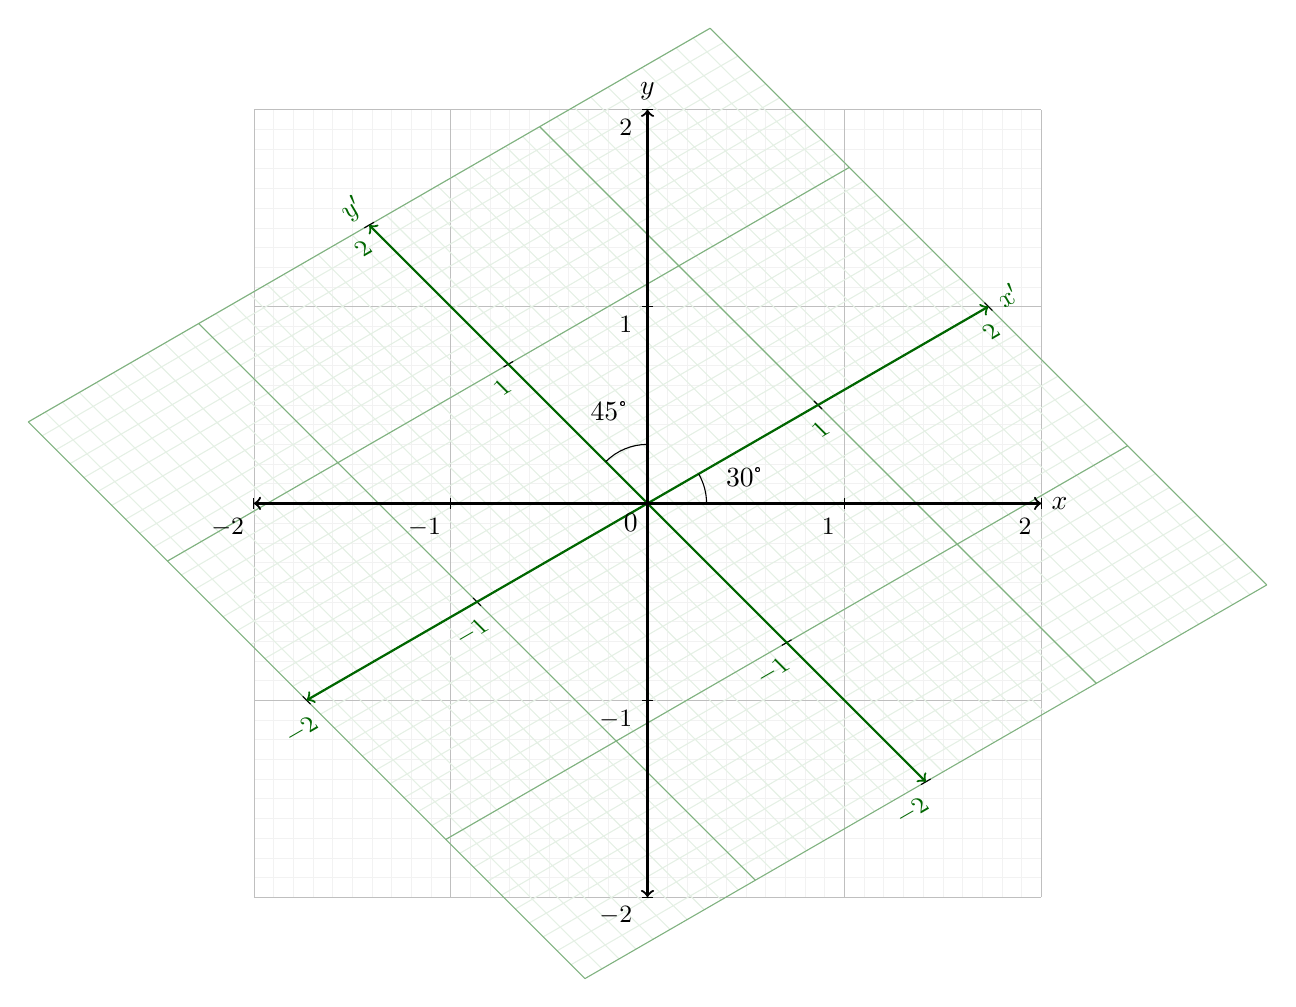
\begin{tikzpicture}[x=2.5cm,y=2.5cm]
        \coordinate (Origin) at (0, 0);
        \coordinate (R) at (0.8660, 0.5);
        \coordinate (P) at (1, 0);
        \coordinate (R2) at (-0.707, 0.707);
        \coordinate (P2) at (0, 1);

        % Draw grid
        \draw[gray!10, very thin, step=0.1] (-2, -2) grid (2, 2);
        \draw[gray!50, very thin, step=1] (-2, -2) grid (2, 2);

        \begin{scope}[cm={0.8660, 0.5, -0.707, 0.707,(0,0)}]
            \draw[step=0.1, black!60!green!10, very thin, thin] (-2,-2) grid (2,2);
            \draw[step=1, black!60!green!50, very thin, thin] (-2,-2) grid (2,2);

            \foreach \x in {-2, -1, 1, 2}
            \draw (\x, 2pt) -- (\x, -2pt) node[black!60!green, below left, transform shape] {\small $\x$};
            \foreach \y in {-2, -1, 1, 2}
            \draw (2pt, \y) -- (-2pt, \y) node[black!60!green, below left, transform shape] {\small $\y$};

            \draw[<->, black!60!green, thick] (-2, 0) -- (2, 0) node[right, transform shape] {$x'$};
            \draw[<->, black!60!green, thick] (0, -2) -- (0, 2) node[above, transform shape] {$y'$};

            % \node[circle, fill=black!60!green, inner sep=0pt, minimum size=5pt, transform shape] 
            %     at (1, 0) {};
            % \node[black!60!green, transform shape, above right] at (1, 0) {A'$(1, 0)$};

            % \node[circle, fill=black!60!green, inner sep=0pt, minimum size=5pt, transform shape] 
            %     at (0, 1) {};
            % \node[black!60!green, transform shape, above right] at (0, 1) {B'$(0, 1)$};
        \end{scope}

        % Draw tick marks on the axes
        \foreach \x in {-2, -1, 1, 2}
        \draw (\x, 2pt) -- (\x, -2pt) node[below left] {\small $\x$};
        \foreach \y in {-2, -1, 1, 2}
        \draw (2pt, \y) -- (-2pt, \y) node[below left] {\small $\y$};

        \node[below left] at (0, 0) {$0$};

        % Draw Cartesian axes
        \draw[<->, thick] (-2, 0) -- (2, 0) node[right] {$x$};
        \draw[<->, thick] (0, -2) -- (0, 2) node[above] {$y$};

        \pic[draw, angle radius=0.75cm, angle eccentricity=1.7, "$30$\textdegree"] {angle=P--Origin--R};
        \pic[draw, angle radius=0.75cm, angle eccentricity=1.7, "$45$\textdegree"] {angle=P2--Origin--R2};

        % \node[circle, fill, inner sep=0pt, minimum size=5pt] 
        %     at (1, 0) {};
        % \node[above right] at (1, 0) {A$(1, 0)$};

        % \node[circle, fill, inner sep=0pt, minimum size=5pt] 
        %     at (0, 1) {};
        % \node[above right] at (0, 1) {B$(0, 1)$};

        % \draw[->, red, line width=0.6mm, >={stealth}] (0, 0) -- (P);
        % \draw[->, black!60!green, line width=0.6mm, >={stealth}] (0, 0) -- (R);

        % \draw[->, red, line width=0.6mm, >={stealth}] (0, 0) -- (P2);
        % \draw[->, black!60!green, line width=0.6mm, >={stealth}] (0, 0) -- (R2);
    \end{tikzpicture}
    \caption{ Overlay of new cartesian plane (green) with axes $x'$ and $y'$
        rotated 30\textdegree\space anti-clockwise and 45\textdegree\space anti-clockwise respectively. }
    \label{2d_axis_shear}
\end{figure}

Figure \ref{2d_axis_shear} depicts what is known as a "shear". It occurs when
each axis is rotated by a different angle, and results in warping of the
transformed vectors, evident by the asymmetric appearance of the graph. Using a
particular set of shears, it is technically possible to skew, flip, scale and
even rotate any set of points in 2D space. As an aside, one might find it
interesting that rotations are nothing more than two shears applied on different
axes by an equal angle. \\ 

The elegance in this model comes from how one such transformation is actually
computed. The first step to this is determining the direction and dilation of
the transformed axes by examining what one desires to happen to the vectors
$\begin{bmatrix} 1 \\
        0\end{bmatrix}$ and $\begin{bmatrix} 0 \\
        1\end{bmatrix}$ after the transformation. Because these vectors each lie
in their respective axis, if the magnitude of any one of them changes, that
means that that axis has been dilated by a factor of the magnitude. If the
direction changes, that means that that axis has been rotated. By knowing the
final position of these two vectors after a transformation, the transformation
that took place can be reconstructed and applied to more points. This means that
if one computes the transformation of just these two vectors once, the
transformation can be inexpensively reapplied to a very large number of points,
and this is the key reason why transformation matrices are used today.

\pagebreak

Now that we understand the theory of axis shifting, we can look at how this can
be represented mathematically using ``transformation matrices". Effectively,
transformation matrices represent a transformation which can be applied to a set
of points. 2D transformation matrices are constructed by taking the ``axial
vectors" discussed above and storing them in a 2$\times$2 matrix. This allows us
to represent any 2D transformation as a matrix multiplication. \\

Let $\vec{x}$ be the position of $\begin{bmatrix} 1 \\ 0
    \end{bmatrix}$ after transformation: $\vec{x} = \begin{bmatrix} x_x \\ x_y \end{bmatrix}$ 
    
Let $\vec{y}$ be the position of $\begin{bmatrix} 0 \\ 1\end{bmatrix}$ after the transformation: $\vec{y} =
    \begin{bmatrix}y_x \\ y_y \end{bmatrix}$
    
The transformation matrix $M$ is therefore described by $M = \begin{bmatrix} x_x & y_x \\
                x_y & y_y
    \end{bmatrix}$.\\

The transformation $T_M(\vec{v})$ of point vector $\vec{v} = \begin{bmatrix}v_x \\ v_y \end{bmatrix}$ using $M$ can then
be described by

\begin{align*}
    T_M(\vec{v}) = M\vec{v} = 
    \begin{bmatrix}
        x_x & y_x \\
        x_y & y_y
    \end{bmatrix}
    \begin{bmatrix}
        v_x \\
        v_y
    \end{bmatrix}
    =
    \begin{bmatrix}
        x_xv_x + y_xv_y \\
        x_yv_x + y_yv_y
    \end{bmatrix}
\end{align*}

If $\vec{x}$ and $\vec{y}$ do not change after a transformation, they would be
equal to $\begin{bmatrix} 1 \\ 0 \end{bmatrix}$ and $\begin{bmatrix} 0 \\ 1
\end{bmatrix}$ respectively. In this state, they are called the ``identity
vectors'' $\vec{x}_i$ and $\vec{y}_i$. From this, a transformation matrix which
does nothing (similarly called the ``identity matrix'') $I$ can be constructed in the form
$
    I = \begin{bmatrix}
        1 & 0 \\
        0 & 1
    \end{bmatrix}
$. In this case, $
T_{I}(\vec{v}) 
= \begin{bmatrix}
    x_{ix} & y_{ix} \\
    x_{iy} & y_{iy}
\end{bmatrix}
\begin{bmatrix}
    v_x \\
    v_y
\end{bmatrix}
= \begin{bmatrix}
   1 & 0 \\
   0 & 1
\end{bmatrix}
\begin{bmatrix}
    v_x \\
    v_y
\end{bmatrix}
= \begin{bmatrix}
        (1)v_x + (0)v_y \\
        (0)v_x + (1)v_y 
\end{bmatrix}
= \begin{bmatrix}
    v_x \\
    v_y
\end{bmatrix} 
= \vec{v}$. \\\\

\pagebreak

    \begin{figure}[H]
        \centering

        \subfloat[\centering Rotation of $\begin{bmatrix}1 \\ 0\end{bmatrix}$ by
        angle $\theta$ from the x-axis.]{
            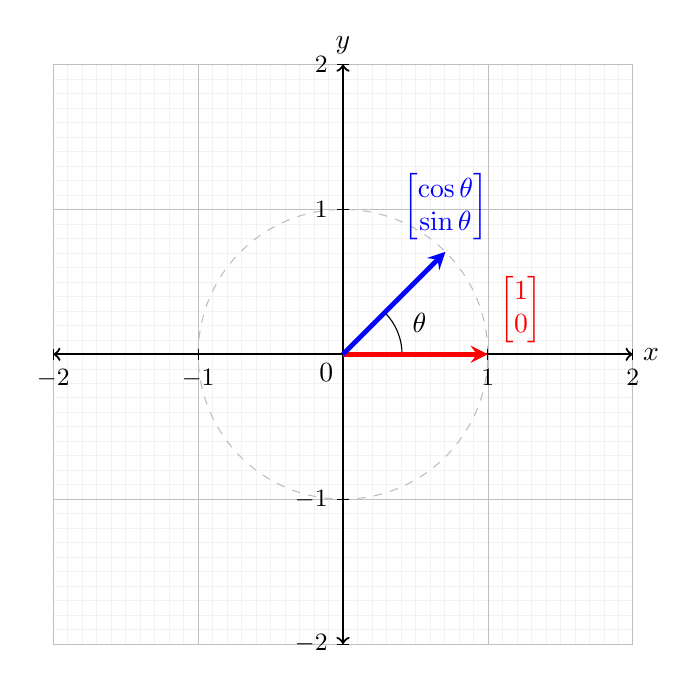
\begin{tikzpicture}[x=1.84cm,y=1.84cm]
                \coordinate (Origin) at (0, 0);
                \coordinate (R) at (0.7071, 0.7071);
                \coordinate (P) at (1, 0);
        
                % Draw grid
                \draw[gray!10, very thin, step=0.1] (-2, -2) grid (2, 2);
                \draw[gray!50, very thin, step=1] (-2, -2) grid (2, 2);
        
                \draw[gray!50, dashed] (0, 0) circle (1);
        
                % Draw tick marks on the axes
                \foreach \x in {-2, -1, 1, 2}
                \draw (\x, 2pt) -- (\x, -2pt) node[below] {\small $\x$};
                \foreach \y in {-2, -1, 1, 2}
                \draw (2pt, \y) -- (-2pt, \y) node[left] {\small $\y$};
        
                \node[below left] at (0, 0) {$0$};
        
                % Draw Cartesian axes
                \draw[<->, thick] (-2, 0) -- (2, 0) node[right] {$x$};
                \draw[<->, thick] (0, -2) -- (0, 2) node[above] {$y$};
        
                \pic[draw, angle radius=0.75cm, angle eccentricity=1.4, "$\theta$"] {angle=P--Origin--R};
        
                % Draw red vector arrow [1, 0]
                \draw[->, red, line width=0.6mm, >={stealth}] (0, 0) -- (P) node[above right] {$\begin{bmatrix}1 \\ 0\end{bmatrix}$};
        
                % Draw blue vector arrow [0.7071, 0.7071]
                \draw[->, blue, line width=0.6mm, >={stealth}] (0, 0) -- (R) node[above]
                    {$\begin{bmatrix}\cos \theta \\ \sin \theta\end{bmatrix}$};
        
            \end{tikzpicture}
        }
        \qquad
        \subfloat[\centering Rotation of $\begin{bmatrix}0 \\ 1\end{bmatrix}$ by
        angle $\theta$ from the y-axis.]{
            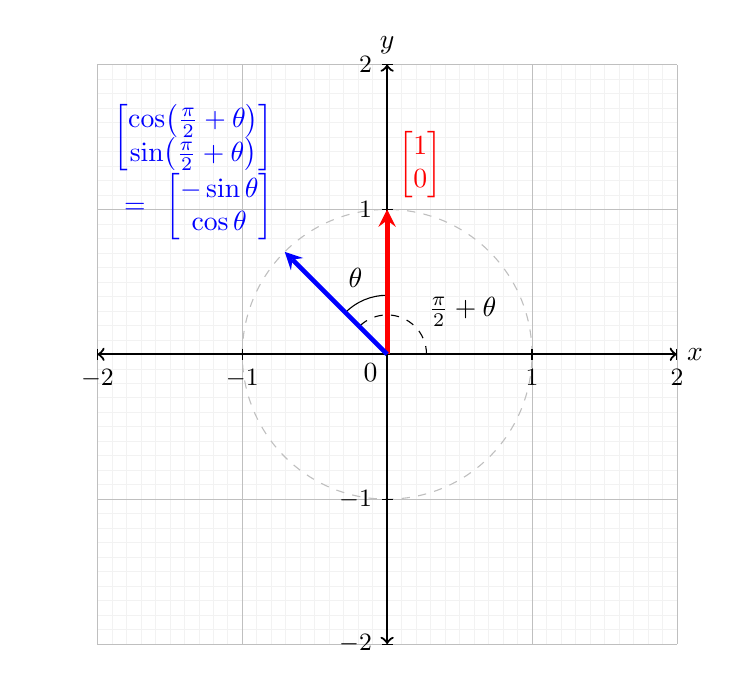
\begin{tikzpicture}[x=1.84cm,y=1.84cm]
                \coordinate (Origin) at (0, 0);
                \coordinate (R) at (-0.7071, 0.7071);
                \coordinate (P) at (0, 1);
                \coordinate (S) at (1, 0);
        
                % Draw grid
                \draw[gray!10, very thin, step=0.1] (-2, -2) grid (2, 2);
                \draw[gray!50, very thin, step=1] (-2, -2) grid (2, 2);
        
                \draw[gray!50, dashed] (0, 0) circle (1);
        
                % Draw tick marks on the axes
                \foreach \x in {-2, -1, 1, 2}
                \draw (\x, 2pt) -- (\x, -2pt) node[below] {\small $\x$};
                \foreach \y in {-2, -1, 1, 2}
                \draw (2pt, \y) -- (-2pt, \y) node[left] {\small $\y$};
        
                \node[below left] at (0, 0) {$0$};
        
                % Draw Cartesian axes
                \draw[<->, thick] (-2, 0) -- (2, 0) node[right] {$x$};
                \draw[<->, thick] (0, -2) -- (0, 2) node[above] {$y$};
        
                \pic[draw, angle radius=0.75cm, angle eccentricity=1.4, "$\theta$"] {angle=P--Origin--R};
                \pic[draw, dashed, angle radius=0.5cm, angle eccentricity=1.6,
                "$\frac{\pi}{2} + \theta$", pic text options={shift={(0.65cm,-0.2cm)}}] {angle=S--Origin--R};
        
                % Draw red vector arrow [1, 0]
                \draw[->, red, line width=0.6mm, >={stealth}] (0, 0) -- (P) node[above right] {
                    $\begin{bmatrix}1 \\ 0\end{bmatrix}$};
        
                % Draw blue vector arrow [0.7071, 0.7071]
                \draw[->, blue, line width=0.6mm, >={stealth}] (0, 0) -- (R)
                node[above left, text width=3cm, align=right] {
                    $\begin{bmatrix}
                        \cos (\frac{\pi}{2} + \theta) \\ 
                        \sin (\frac{\pi}{2} + \theta)
                    \end{bmatrix}$
                    $= \begin{bmatrix} -\sin\theta \\
                        \cos\theta \end{bmatrix}$
                };
        
            \end{tikzpicture}
        }

        \caption{Rotation of the 2D axes by angle $\theta$ anti-clockwise.}
        \label{2d_ax_rot}
    \end{figure}

As seen in Figure \ref{2d_ax_rot}, on a unit circle, a counter-clockwise
rotation of the identity position vector $\vec{x}_i = \begin{bmatrix} 1 \\ 0
\end{bmatrix}$ by $\theta$ would be represented as $\vec{x} = \begin{bmatrix}
\cos\theta \\
\sin\theta \end{bmatrix}$. Likewise, the rotation of the identity position
vector $\vec{y}_i = \begin{bmatrix} 0 \\ 1 \end{bmatrix}$ would be equrivalent to first
rotating by $\frac{\pi}{2}$ and then by $\theta$, hence $\vec{y} =
\begin{bmatrix} \cos (\frac{\pi}{2} + \theta) \\
    \sin (\frac{\pi}{2} + \theta) \end{bmatrix} = \begin{bmatrix} -\sin\theta \\
\cos\theta \end{bmatrix}$. Hence, a 2D transformation matrix $R(\theta)$ can be
constructed so that it rotates the 2D axes by an angle $\theta$ using $\vec{x}$
and $\vec{y}$. This is what is known as a rotation matrix.

\begin{align*}
    R(\theta) & = \begin{bmatrix}
                      \cos\theta & -\sin\theta \\
                      \sin\theta & \cos\theta
                  \end{bmatrix}
\end{align*}

% TODO: needs clarity
You can combine different linear transformations by multiplying a vector by
multiple transformation matrices sequentially. For example, you might choose to
apply a shear or a scale to your points before rotating them. This property
applies to both two and three dimensional transformation matrices. Because of
this versatility, transformation matrices are very easy to work with and
integrate into more complex applications where multiple transformations need to
be chained. \\

It is important to note that matrix multiplication is not commutative, and hence
it is important to always multiply matrices in a right-to-left order: if one
wanted to apply the linear transformations $T_1 \to T_2 \to T_3$ on vector
$\vec{v}$, the correct multiplication would be $T_3T_2T_1\vec{v}$.
\pagebreak
\subsection{In three dimensions}
Now that we have established basic intuition on what 2D matrices transformation
allow us to do, we can extend the established observations to three dimensions.
\\

In 3D, there are now three axes which must be kept track of:
\begin{itemize}[leftmargin=2cm]
    \item X (left $\leftrightarrow$ right)
    \item Y (forward $\neswarrow$ back)
    \item Z (up $\updownarrow$ down)
\end{itemize}

The identity vectors $\vec{x}_0$, $\vec{y}_0$ and $\vec{z}_0$ in three
dimensions, like we saw with 2D, have a magnitude of $1$ and lie on the axis
they represent.

\begin{align*}
    \vec{x}_0 = \begin{bmatrix} 1 \\ 0 \\ 0 \end{bmatrix}
    \quad
    \vec{y}_0 = \begin{bmatrix} 0 \\ 1 \\ 0 \end{bmatrix}
    \quad
    \vec{z}_0 = \begin{bmatrix} 0 \\ 0 \\ 1 \end{bmatrix}
\end{align*} \\

A 3D transformation defines the transition from the identity vectors into ones
($\vec{x}$, $\vec{y}$ and $\vec{z}$) with potentially different magnitude and
direction, signifying reoriented axes.

\begin{align*}
    \vec{x} = \begin{bmatrix}
                  {x}_x \\ {y}_x \\ {z}_x
              \end{bmatrix}
    \quad
    \vec{y} = \begin{bmatrix}
                  {x}_y \\ {y}_y \\ {z}_y
              \end{bmatrix}
    \quad
    \vec{z} = \begin{bmatrix}
                  {x}_z \\ {y}_z \\ {z}_z
              \end{bmatrix}
\end{align*}

Changing the magnitude and/or direction of these vectors results in various
effects on the 3D space, similar to how this works in two dimensions.
Individually changing any one or two of these vectors results in the three
dimensional equrivalent of shear called ``deformation" as the three axes would
no longer be orthogonal, therefore appearing to ``crush'' points within them.
This property is often used in 3D animation to compress or stretch objects -- a
ball hitting a wall, or human skin stretching, for example. \\

As before, constructing a matrix out of these vectors allows us to leverage
matrix multiplication to transform points. A 3$\times$3 matrix $M$ can now be
constructed to represent a 3D transformation using the above axes. Hence, the
identity 3D rotation matrix $M_0$ can also be defined here.

\begin{align*}
    M = \begin{bmatrix}
            {x}_x & {y}_x & {z}_x \\
            {x}_y & {y}_y & {z}_y \\
            {x}_z & {y}_z & {z}_z
        \end{bmatrix} \quad\therefore\quad M_0 = \begin{bmatrix}
                                                     1 & 0 & 0 \\
                                                     0 & 1 & 0 \\
                                                     0 & 0 & 1
                                                 \end{bmatrix}
\end{align*}

For a transformation $T_M(\vec{v})$ on $\vec{v} = \begin{bmatrix}
        v_x \\
        v_y \\
        v_z \end{bmatrix}$ by matrix $M$,

\begin{align*}
    T_M(\vec{v}) = M\vec{v} = \begin{bmatrix}
                                  {x}_x & {y}_x & {z}_x \\
                                  {x}_y & {y}_y & {z}_y \\
                                  {x}_z & {y}_z & {z}_z
                              \end{bmatrix}
    \begin{bmatrix}
        v_x \\
        v_y \\
        v_z
    \end{bmatrix}
    =
    \begin{bmatrix}
        x_x v_x + y_x v_y + z_x v_y \\
        x_y v_x + y_y v_y + z_y v_y \\
        x_z v_x + y_z v_y + z_z v_y \\
    \end{bmatrix}
\end{align*}

Now that we are familiar with the form of a 3D rotation matrix, we can move on
to methods of constructing one. In a sense, one could say simply knowing how to
use a rotation matrix to transform points is rather useless without knowing how
to construct the rotation matrix in the first place. Historically, many
construction methods have been invented and used widely, each with their own
benefits and shortcomings.

It is interesting to note that while I initially wanted to compare rotation
matrices as a whole to quaternion rotation, this fact occurred to me and I
realised that it would be more appropriate to compare the most popular
construction method of rotation matrices to quaternion rotation instead. 

\subsection{Construction from Euler angles}

\subsubsection{Concept}
In real life, it is practical to represent rotations with easily measurable
metrics, like angles. Aircraft and watercraft make extensive use of yaw, pitch
and roll angles in instrumentation to aid their pilots in judging the
orientation of the craft. Yaw indicates the left-right angle of the nose,
rotating about the vertical axis, somewhat like the ``heading'' of aircraft. A
yaw of 0\textdegree\space indicates the nose is pointing directly north, and a
yaw of 90\textdegree\space indicates the nose is pointing directly east, etc.
Pitch indicates the angle of the nose relative to the horizon, and roll
indicates how much the plane is turned about the forward axis. Figure
\ref{yawpitchroll} demonstrates this in terms of an $x$, $y$ and $z$ axis. In
aircraft, $y$ axis here can be considered the ``front'' of the craft, the $z$
axis the ``up'' direction and the $x$ axis the ``right'' direction. \\

\begin{figure}[H]
    \centering
    \tdplotsetmaincoords{70}{-45}
    \begin{tikzpicture}[x=0.5cm,y=0.5cm,z=0.3cm,>=stealth,tdplot_main_coords]
        \coordinate (X) at (3,0,0);
        \coordinate (Y) at (0,3,0);
        \coordinate (Z) at (0,0,3);

        \draw[->, black!30!red] (0,0,0) -- (X) node[right] {$x$};
        \draw[->, black!30!blue] (0,0,0) -- (Y) node[left] {$y$};
        \draw[->, black!30!green] (0,0,0) -- (Z) node[above] {$z$};

        \node[red] at (2.25,0,0.8) {$pitch$};
        \begin{scope}[canvas is zy plane at x=2.5]
            \draw[red, dashed] (0,0) circle (0.3);
        \end{scope}

        \node[black!30!green] at (1,0,2.25) {$yaw$};
        \begin{scope}[canvas is xy plane at z=2.5]
            \draw[black!30!green, dashed] (0,0) circle (0.3);
        \end{scope}

        \node[blue] at (0.1,2.25,0.6) {$roll$};
        \begin{scope}[canvas is xz plane at y=2]
            \draw[blue, dashed] (0,0) circle (0.3);
        \end{scope}


    \end{tikzpicture}
    \caption{Yaw pitch and roll}
    \label{yawpitchroll}
\end{figure}

Euler angles are based around this concept. A set of Euler angles is a 3D vector
containing the yaw, pitch and roll of an object around a reference frame. In the
example of aircraft, the reference frame is usually the surface of the Earth. In
space, it is usually a prominent constellation or celestial object. If one
wishes to encode a rotation as a set of Euler angles, one just needs to measure
the angles between the rotated axes and the original axes of the reference
frame. \\

As this system of representing rotation is simple, measurable and intuitive for
humans to use, one of the main ways of constructing a rotation matrix is through
Euler angles.

\pagebreak
\subsubsection{Deriving rotation matrices for each angle}
\label{section_deriving_rot_for_each_angle}
Consider rotating the 3D identity axes with vectors $\vec{x}_0$, $\vec{y}_0$ and
$\vec{z}_0$ by $\theta$ around the X axis. Let the matrix that describes this
rotation in terms of $\theta$ be $R_x(\theta)$. After the transformation, let
the identity vectors' new positions be $\vec{x}_r$, $\vec{y}_r$ and $\vec{z}_r$.
\\

% TODO: insert figure

\begin{figure}[H]
    \centering
    \tdplotsetmaincoords{70}{50}
    \begin{tikzpicture}[x=0.5cm,y=0.5cm,z=0.3cm,>=stealth,tdplot_main_coords]
        \coordinate (X) at (5,0,0);
        \coordinate (Y) at (0,3,0);
        \coordinate (Z) at (0,0,3);

        \draw[->, red] (0,0,0) -- (X) node[right] {$\vec{x}_r = R_{x}(\theta)\cdot \vec{x}_0 = x_0$};
        \draw[->, blue] (0,0,0) -- (Y) node[right] {$\vec{y}_0$};
        \draw[->, black!60!green] (0,0,0) -- (Z) node[above] {$\vec{z}_0$};

        \begin{scope}[canvas is zy plane at x=0]
            \draw[dashed, darkgray] (0,0) circle (3);
            \draw[->, blue, dashed] (0,0) -- ({sin(20)*3}, {cos(20)*3}) node[right] {$\vec{y}_r = R_{x}(\theta)\cdot \vec{y}_0$};
            \draw[->, black!60!green, dashed] (0,0) -- ({sin(110)*3}, {cos(110)*3}) node[above left] {$\vec{z}_r = R_{x}(\theta)\cdot \vec{z}_0$};

            \draw[black!30!blue] (0.26,1.5) node {$\theta$};
            \draw[black!80!green] (1.5,-0.26) node {$\theta$};
        \end{scope}

    \end{tikzpicture}
    \caption{Rotation around the X-axis by angle $\theta$. $\vec{x}_r$,
        $\vec{y}_r$ and $\vec{z}_r$ represent the identity vectors after the
        transformation by $R_x(\theta)$ where $\vec{x}_0 \to \vec{x}_r$,
        $\vec{y}_0 \to \vec{y}_r$ and $\vec{z}_0 \to \vec{z}_r$.}
    \label{3d_euler_rot_x}
\end{figure}

Considering the components of $\vec{x}_r$, $\vec{y}_r$ and $\vec{z}_r$,

\begin{align*}
    \vec{x}_r = \begin{bmatrix} {x}_{rx} \\ {x}_{ry} \\ {x}_{rz} \end{bmatrix} \quad
    \vec{y}_r = \begin{bmatrix} {y}_{rx} \\ {y}_{ry} \\ {y}_{rz} \end{bmatrix} \quad
    \vec{z}_r = \begin{bmatrix} {z}_{rx} \\ {z}_{ry} \\ {z}_{rz} \end{bmatrix}
\end{align*}

Hence, in Figure \ref{3d_euler_rot_x}, the rotation $R_x(\theta)$ could be represented
as

\begin{align*}
    R_x(\theta) = \begin{bmatrix}
        {x}_{rx} & {y}_{rx} & {z}_{rx} \\
        {x}_{ry} & {y}_{ry} & {z}_{ry} \\
        {x}_{rz} & {y}_{rz} & {z}_{rz}
    \end{bmatrix}
\end{align*}\\

From Figure \ref{3d_euler_rot_x} it becomes apparent that points that lie along
$\vec{x}_0$ do not move at all, because the rotation is happening around
$\vec{x}_0$ in the first place. Hence,

\begin{align*}
    \vec{x}_r = \vec{x}_0 = \begin{bmatrix} 1 \\
                              0 \\ 0\end{bmatrix}
\end{align*}

Points colinear with the Y axis get rotated around a unit circle in the YZ plane
(pictured in Figure \ref{3d_euler_rot_x}). Hence, $\vec{y}_r$ is described with
the trigonometric functions $\cos \theta$ and $\sin \theta$ as its Y and Z
components. The rotation of $\vec{z}_r$ can be derived similarly.

\begin{align*}
    \vec{y}_r = \begin{bmatrix} 0 \\ \cos\theta \\ \sin\theta
                      \end{bmatrix}
    \quad
    \vec{z}_r
    = \begin{bmatrix}
          0           \\
          -\sin\theta \\
          \cos\theta
      \end{bmatrix}
\end{align*}

Combining $\vec{x}_r, \vec{y}_r$ and $\vec{z}_r$ yields the rotation matrix
$R_x(\theta)$ for rotations around the X-axis.

\begin{align*}
    R_x(\theta)
    = \begin{bmatrix}
          1 & 0          & 0           \\
          0 & \cos\theta & -\sin\theta \\
          0 & \sin\theta & \cos\theta
      \end{bmatrix}
\end{align*}

A  similar process can be followed to derive the rotation matrices by the Y and
Z axes, so it has been omitted for brevity. The only thing that changes in the
derivation process is that the plane of the circle always lies in the plane
described by the two axes perpendicular to the rotation axis.

\begin{align*}
    R_y(\theta) = \begin{bmatrix}
                      \cos \theta  & 0 & \sin \theta \\
                      0            & 1 & 0           \\
                      -\sin \theta & 0 & \cos \theta
                  \end{bmatrix}
    \quad
    R_z(\theta) = \begin{bmatrix}
                      \cos \theta & -\sin \theta & 0 \\
                      \sin \theta & \cos \theta  & 0 \\
                      0           & 0            & 1
                  \end{bmatrix}
\end{align*}

\subsubsection{Multiplication}

It is now possible to compute a rotation matrix in terms of the Euler angles
$\alpha$, $\beta$ and $\gamma$ (representing pitch, roll and yaw respectively)
by first constructing each individual matrix, then multiplying them.
Effectively, this applies the rotation $R_x(\alpha)$ followed by $R_y(\beta)$
and finally $R_z(\gamma)$.

\begin{align*} \\
    R(\alpha, \beta, \gamma) & = R_z(\gamma) R_y(\beta) R_x(\alpha)                                                                                                \\
                             & = \begin{bmatrix}
                                     \cos \gamma & -\sin \gamma & 0 \\
                                     \sin \gamma & \cos \gamma  & 0 \\
                                     0           & 0            & 1 \\
                                 \end{bmatrix}
    \begin{bmatrix}
        \cos \beta  & 0 & \sin \beta \\
        0           & 1 & 0          \\
        -\sin \beta & 0 & \cos \beta \\
    \end{bmatrix}
    \begin{bmatrix}
        1 & 0           & 0            \\
        0 & \cos \alpha & -\sin \alpha \\
        0 & \sin \alpha & \cos \alpha  \\
    \end{bmatrix}                                                                                                                                 \\
                             & = \begin{bmatrix}
                                     \cos\beta\cos\gamma & \sin\alpha\sin\beta\cos\gamma - \cos\alpha\sin\gamma & \cos\alpha\sin\beta\cos\gamma + \sin\alpha\sin\gamma \\
                                     \cos\beta\sin\gamma & \sin\alpha\sin\beta\sin\gamma + \cos\alpha\cos\gamma & \cos\alpha\sin\beta\sin\gamma - \sin\alpha\cos\gamma \\
                                     -\sin\beta          & \sin\alpha\cos\beta                                  & \cos\alpha\cos\beta                                  \\
                                 \end{bmatrix}
\end{align*} \\

As matrix multiplication does not commute, it is not always the case that
rotating by an axis A, then rotating by B would be the same as rotating first by
axis B, then by A. Hence, it is important to note that the order of
multiplication of $R_z$, $R_y$ and $R_x$ produces a unique final rotation. For
the rest of the investigation, the $x \to y \to z$ rotation order seen above
will be used. This is alternatively called the ZYX Tait-Bryan order (Wikipedia
Contributors, 2023). \\

It is important to note that traditionally, there has been no set standard
defining which rotation order to use - this is left up to choice. In 3D software
which uses Euler angles, it is still required to manually specify the order of
rotation. When working with large teams of people, such as in an animation and
game development studio, or a scientific research team, it is still required to
agree on a standard order of Euler angles to avoid ambiguity and
misunderstanding, which is potentially a weakness of using the Euler angle
system in the first place. \\

\pagebreak
\subsection{The gimball lock problem}
There is another large problem with constructing rotation matrices from Euler
angles. Suppose you rotated an object with the Euler angles
$\alpha$, $\beta$ and $\gamma$, where $\beta=\frac{\pi}{2}$

\begin{align*} \\
    R(\alpha, \frac{\pi}{2}, \gamma)
     & = \begin{bmatrix}
             \cos\frac{\pi}{2}\cos\gamma & \sin\alpha\sin\frac{\pi}{2}\cos\gamma - \cos\alpha\sin\gamma & \cos\alpha\sin\frac{\pi}{2}\cos\gamma + \sin\alpha\sin\gamma \\
             \cos\frac{\pi}{2}\sin\gamma & \sin\alpha\sin\frac{\pi}{2}\sin\gamma + \cos\alpha\cos\gamma & \cos\alpha\sin\frac{\pi}{2}\sin\gamma - \sin\alpha\cos\gamma \\
             -\sin\frac{\pi}{2}          & \sin\alpha\cos\frac{\pi}{2}                                  & \cos\alpha\cos\frac{\pi}{2}                                  \\
         \end{bmatrix}
    \\
    &\text{Substituting $\cos\frac{\pi}{2} = 0$ and $\sin\frac{\pi}{2} = 1$:} \\
     & = \begin{bmatrix}
             0  & \sin\alpha\cos\gamma - \cos\alpha\sin\gamma & \cos\alpha\cos\gamma + \sin\alpha\sin\gamma \\
             0  & \sin\alpha\sin\gamma + \cos\alpha\cos\gamma & \cos\alpha\sin\gamma - \sin\alpha\cos\gamma \\
             -1 & 0                                           & 0                                           \\
         \end{bmatrix}
    \\
    &\text{Applying trigonometric identities:} \\
     & = \begin{bmatrix}
             0  & \sin(\alpha - \gamma) & \cos(\alpha - \gamma)  \\
             0  & \cos(\alpha - \gamma) & -\sin(\alpha - \gamma) \\
             -1 & 0                     & 0                      \\
         \end{bmatrix}
\end{align*} \\

Let $\alpha - \gamma = \theta$. The rotation matrix $R$ can now be expressed as
$R(\theta) =
    \begin{bmatrix} 0  & \sin\theta & \cos\theta  \\
    0  & \cos\theta & -\sin\theta \\
    -1 & 0          & 0           \\
\end{bmatrix}$.\\
By inspecting this matrix, we find that:

\begin{itemize}[leftmargin=2cm]
    \item $\vec{x_0}$ will always transform to $\begin{bmatrix} 0 \\ 0 \\ -1
    \end{bmatrix} = -\vec{z_0}$. This means that this is the axis around which
    rotation occurs by angle $\theta$ as it remains constant irrespective of the
    value of $\theta$.
    \item $\vec{y}$ and $\vec{z}$ revolve around a unit circle in the YX plane
    by angle $\theta$ perpendicularly to the axis of rotation of $-\vec{z_0}$,
    as seen before in Figure \ref{3d_euler_rot_x}.
    \item This matrix is entirely in terms of $\theta$. When either $\alpha$ or
    $\gamma$ is changed, the resulting rotation is always around the
    $-\vec{z_0}$ axis as it is independent of $\theta$.
\end{itemize}

Hence, this shows that when $\beta = \frac{\pi}{2}$, the rotation matrix
actually loses one degree of rotational freedom entirely as $\alpha$ and
$\gamma$ describe rotation about the same axis because they both contribute to
the value of $\theta$. In fact, the same can be shown for the case where one of
$\alpha$, $\beta$ or $\gamma$ is equal to $\frac{(2b+1)\pi}{2}$ where $b \in
\mathbb{Z}$. \\

This phenomenon is known as "gimball lock". It is widely considered to be one of
the largest issues with using Euler angles for rotation. It is significant
because it means that for specific angles of rotation, the system can actually
lose the ability to freely rotate, and may even be unable to escape the gimball
lock. \\

\pagebreak

\begin{figure}[H]
    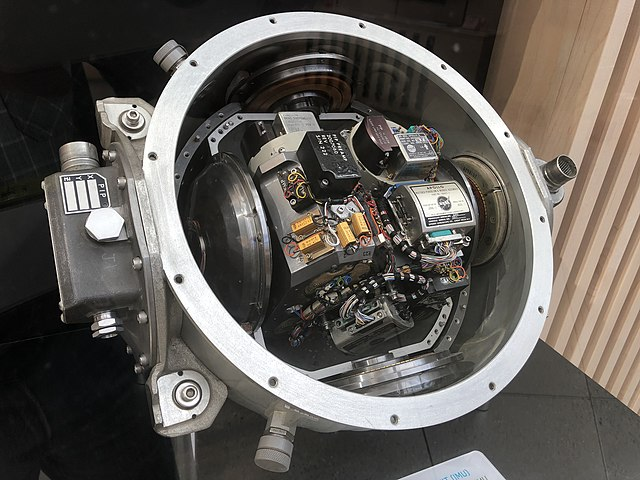
\includegraphics[width=8cm]{res/apollo_imu.jpg}
    \centering
    \caption{The Apollo 11 "Inertial Measurement Unit" responsible for guidance \& orientation of the spacecraft in space.}
\end{figure}

One of the most famous examples of gimball lock in action was during the 1969
Apollo 11 manned mission to the moon. The Apollo 11 spacecraft was equipped with
an "Inertial Measurement Unit" which was responsible for measuring the
orientation of the spacecraft in space. This was done using three gyroscopes,
each of which measured the rotation of the spacecraft in terms of yaw, pitch and
roll relative to the craft's starting position. Mechanically, these gyroscopes,
too undergo gimball lock when the spacecraft is oriented at specific angles
resulting in complete disorientation of the guidance unit. This happened
in-flight during the actual mission, meaning that the unit had to be manually
moved out of the gimbal lock position using the stars as a reference, in order
to regain the lost degree of freedom. \\

This fundamental flaw with Euler angles demonstrates how despite their
simplicity and intuitiveness, they clearly leave a lot to be desired for
rigorously representing 3D rotations. \\

% \subsection{The spherical linear interpolation problem}

\section{Improving on Euler angles with Quaternions}
In 1843, Irish mathematician Sir William Rowan Hamilton proposed an alternative
way to represent 3D rotation by using four dimensional imaginary numbers called
"quaternions". Quaternions allow us to rotate any 3D position vector around any
3D axis by a certain angle with the power of four dimensions (Dam, Koch and
Lillholm, 1998). Rotation about an axis is not anything special in particular,
in fact, rotating around the X, Y and Z axes individually has already been
explored in section \ref{section_deriving_rot_for_each_angle}. \\

Quaternions, like rotation matrices constructed from Euler angles, have seen
numerous applications in pretty nearly all fields of science and engineering
where 3D rotations are required. As we will soon see, quaternions address many
of the downsides of Euler angle matrices, and can often be a very efficient
alternative to them.

\pagebreak

\subsection{Hamilton's Definition}
Quaternions, like complex numbers, are defined with "real" and "imaginary"
parts, and are essentially an extension of the complex numbers to four
dimensions. The set of all quaternions is known as $\mathbb{H}$, named after
Hamilton. Algebraically, a quaternion $q$ can be defined in terms of the
coefficients of its terms:

\begin{align*}
    q = a + bi + cj + dk \quad a, b, c, d \in \mathbb{R}
\end{align*}

$i$, $j$ and $k$, called "basic quaternions", do not have an explicit definition
of their value but are rather defined expressly in terms of the way they
interact with each other in that they must satisfy the equality

\begin{align*}
    i^2 = j^2 = k^2 = ijk = -1
\end{align*}

\qquad\qquad\qquad\qquad\qquad\qquad\qquad\qquad\qquad\qquad\qquad\qquad\qquad\qquad\qquad
(Dam, Koch and Lillholm, 1998).

\subsection{Basic Quaternions}
In order to start using quaternions for rotation, we must first explore the
details that their definition implies. We must first define how $i$, $j$, and
$k$ interact algebraically, as this will be the basis for many of the
quaternion's properties.
\subsubsection{Multiplying by Real Numbers}
For any $n \in \mathbb{R}$, it is defined that $in = ni$, $jn = nj$ and $kn =
    nk$. Hence, for any $q \in \mathbb{H}$, $qn = nq$. Quaternion multiplication by
real numbers does, in fact, commute (Dam, Koch and Lillholm, 1998).

\subsubsection{Multiplication by other basic quaternions}
Hamilton's quaternion definition can then be used to derive the multiplicative
interactions between $i$, $j$ and $k$:

% ij & jk
\begin{align*}
     &
    \begin{aligned}
        ijk    & = k^2   \\
        ijk^2  & = k^2k  \\
        ij(-1) & = (-1)k \\
        ij     & = k
    \end{aligned}
     &
    \begin{aligned}
        ijk    & = i^2         \\
        i^2 jk & = i \cdot i^2 \\
        (-1)jk & = i(-1)       \\
        jk     & = i
    \end{aligned}
\end{align*}

% kj and ji
\begin{align*}
     &
    \begin{aligned}
        i  & = jk   \\
        ji & = j^2k \\
        ji & = -k
    \end{aligned}
     &
    \begin{aligned}
        k  & = ij   \\
        kj & = ij^2 \\
        kj & = -i
    \end{aligned}
\end{align*}

% ki & ik
\begin{align*}
     &
    \begin{aligned}
        ij     & = k     \\
        kij    & = k^2   \\
        kij^2  & = k^2j  \\
        ki(-1) & = (-1)j \\
        ki     & = j
    \end{aligned}
     &
    \begin{aligned}
        k  & = ij   \\
        ik & = i^2j \\
        ik & = -j
    \end{aligned}
\end{align*}

An important concept becomes apparent from the above calculations. Like with
matrices, quaternion multiplication by other quaternions is not commutative,
that is, it can be the case that $q_1q_2 \neq q_2q_1$ where $ q_1,q_2 \in
\mathbb{H}$. For example, it is seen above that while $ij = k$, $ji = -k$. \\

The multiplication table of basic quaternions is hence formed, where the column
represent the left operand and the row represents the right operand in
multiplication.

\begin{center}
    \doublespacing
    \begin{tabular}{ | c | c | c | c | }
        \hline
        $\times$ & $i$  & $j$  & $k$  \\
        \hline
        $i$      & $-1$ & $-k$ & $j$  \\
        \hline
        $j$      & $k$  & $-1$ & $-i$ \\
        \hline
        $k$      & $-j$ & $i$  & $-1$ \\
        \hline
    \end{tabular}
    \captionof{table}{Basic quaternion noncommutative multiplication table}\label{sophisticatedtable}
\end{center}

As an aside, it is perhaps interesting that the noncommutativity of quaternions
and matrices reflects the noncommutativity of rotations in 3D space. It could be
the case that mathematical models used to represent rotations are noncommutative
because the order of rotations themselves matters, and what we see as an
algebraic constraint is a reflection of what is physically possible. \\  

\subsubsection{Associativity}
Quaternion multiplication is associative in that $(q_1 q_2) q_3 = q_1 (q_2 q_3)$
where $q_1,q_2,q_3 \in \mathbb{H}$.
The same property applies for addition, $(q_1 + q_2) + q_3 = q_1 + (q_2 + q_3)$
where $q_1,q_2,q_3 \in \mathbb{H}$.

This associativity allows for application of useful algebraic
techniques like the distributive law.

\subsection{Quaternion Operations}
\subsubsection{Multiplication of non-basic quaternions}
Let $q_1 = a_1 + b_1i + c_1j + d_1k$ and $q_2 = a_2 + b_2i + c_2j + d_2k$ where
$a_1, b_1, c_1, d_1, a_2, b_2, c_2, d_2 \in \mathbb{R}$. The multiplication
$q_1q_2$ can be computed using the distributive law.

\begin{align*}
    q_1q_2 & = (a_1 + b_1i + c_1j + d_1k)(a_2 + b_2i + c_2j + d_2k)    \\
           & = a_1a_2 + a_1b_2i + a_1c_2j + a_1d_2k                    \\
           & + b_1a_2i + b_1b_2i^2 + b_1c_2ij + b_1d_2ik               \\
           & + c_1a_2j + c_1b_2ji + c_1c_2j^2 + c_1d_2jk               \\
           & + d_1a_2k + d_1b_2ki + d_1c_2kj + d_1d_2k^2               \\
           & \text{Applying the basic quaternion rules then}           \\
           & \text{factoring out the real part and $i$, $j$, and $k$,} \\
           & = a_1a_2 - b_1b_2 - c_1c_2 - d_1d_2                       \\
           & + (a_1b_2 + b_1a_2 + c_1d_2 - d_1c_2)i                    \\
           & + (a_1c_2 - b_1d_2 + c_1a_2 + d_1b_2)j                    \\
           & + (a_1d_2 + b_1c_2 - c_1b_2 + d_1a_2)k
\end{align*}

\pagebreak

\subsubsection{Conjugation}
For any quaternion $q = a + bi + cj + dk \quad a, b, c, d \in \mathbb{R}$, its
conjugate $q^*$ is defined as $q^* = a - bi - cj - dk$. \\

\subsubsection{Multiplication by Conjugate}
Suppose one was to multiply a quaternion $q$ by its conjugate $q^*$,
\begin{align*}
    qq^* & = (a + bi + cj + dk)(a - bi - cj - dk)            \\
         & = a^2 - abi - acj - adk                           \\
         & + bia - (bi)^2 - bicj - bidk                      \\
         & + cja - cjbi - (cj)^2 - cjdk                      \\
         & + dka - dkbi - dkcj - (dk)^2                      \\
         & \text{Reordering real coefficients and expanding} \\
         & = a^2 - abi - acj - adk                           \\
         & + abi - b^2i^2 - bcij - bdik                      \\
         & + acj - bcji - c^2j^2 - cdjk                      \\
         & + adk - bdki - cdkj - d^2k^2                      \\
         & \text{Applying basic quaternion rules}            \\
         & = a^2 - abi - acj - adk                           \\
         & + abi + b^2 - bck + bdj                           \\
         & + acj + bck + c^2 - cdi                           \\
         & + adk - bdj + cdi + d^2                           \\
         &\text{Cancelling like terms,}                      \\
         & = a^2 + b^2 + c^2 + d^2                           \\
         \\
         & \text{Additionally, given } a, b, c, d \in \mathbb{R} \\
         & \therefore a^2 + b^2 + c^2 + d^2 \in \mathbb{R}       \\
         & \therefore qq^* \in \mathbb{R}
\end{align*}

Hence, if you multiply a quaternion by its conjugate, the result will always be
a real number and equal to the sum of the squares of its coefficients. \\

\subsubsection{Norm}
The norm of a quaternion $q$ is defined as $|q| = \sqrt{qq^*} = \sqrt{a^2 + b^2
+ c^2 + d^2}$, corresponding to the length of the quaternion in 4D space, coming
from the extension of the Pythagorean theorem in four dimensions. A quaternion
of norm $1$ is called a unit quaternion. It is hence possible to normalize a
quaternion $q$ by dividing it by its norm. If $\hat{q}$ represents the
normalization of $q$, $q \in \mathbb{H}$, $\hat{q} = \frac{q}{|q|}$. \\

% https://www.quora.com/How-do-I-find-the-inverse-of-a-quaternion
\pagebreak

\subsubsection{Inverse}
The inverse $q^{-1}$ of a quaternion $q$ exists such that $qq^{-1} = 1$,
effectively "undoing" any multiplication caused by $q$. The inverse of a
quaternion can be computed using the previosuly established rules.

\begin{align*}
     & qq^{-1} = 1 \Rightarrow q^{-1} = \frac{1}{q}         \\
     & \Rightarrow q^{-1} = \frac{1}{q} \cdot \frac{q^*}{q^*} = \frac{q^*}{qq^*}
    = \frac{q^*}{a^2 + b^2 + c^2 + d^2} = \frac{q^*}{|q|^2}
\end{align*}

In terms of 3D rotations, the inverse of a quaternion allows one to effectively
"reverse" or "undo" a rotation similarly to how multiplying by the inverse of a
transformation matrix reverses the transformation.

\subsection{Rotating position vectors}
Although quaternions harbor many different interesting properties, from the very
beginning, Hamilton defined them out of the need for unit quaternions to
represent 3D rotation in a straightforward manner.

Hamilton's method of rotation involves taking a vector one wishes to rotate, for
example $\vec{v} = \begin{bmatrix} x \\ y \\ z \end{bmatrix}$ and constructing a
quaternion $p$ out of it such that $p = xi + yj + zk$. As the real part $\Re(p)$
of $p$ is zero, $p$ is called a "pure quaternion". \\

Like with rotation matrices, one can then construct a ``rotation quaternion" $q =
a + bi + cj +dk$ that represents a rotation about an axis $\vec{g} =
\begin{bmatrix} b \\ c \\ d \end{bmatrix}$ by an angle $\theta$ as follows. %

% represents a direction in 3D space, and is hence a unit vector. That is,
% $\vec{g} = \vec{\hat{g}}$. \\

Considering that $q$ is a unit quaternion,

\begin{align*}
    &|q| = 1 = |q|^2 = a^2 + b^2 + c^2 + d^2 \\
    &\text{Given that } \sin^2\theta + \cos^2\theta = 1, \\
    &a^2 + (b^2 + c^2 + d^2) = 1 = \sin^2\theta +c \cos^2\theta \\
    &\text{From this, one could infer that} \\
    &a = \cos\theta, \sqrt{b^2 + c^2 + d^2} = |\vec{g}| = \sin\theta \quad or \quad a = \cos\theta, \sqrt{b^2 + c^2 + d^2} = |\vec{g}| = \sin\theta 
\end{align*}

Let $h$ equal a quaternion of the form $h = bi + cj + dk$.
\begin{align*}
    &|\vec{g}| = |h| = \sqrt{b^2 + c^2 + d^2} \\
    &bi + cj + dk = \frac{(bi + cj + dk)}{|\vec{g}|}|\vec{g}| = \frac{h}{|h|}|\vec{g}| = \hat{h}\sin\theta
\end{align*}

Hence, for a rotation by any axis and angle, one can construct a rotation
quaternion $q = \cos\theta + \hat{h}\sin\theta$, where $\theta$ represents the
rotation angle, and $\hat{h}$ represents the normalization of a pure quaternion
of the form $xi + yj + zk$ where $x$, $y$ and $z$ are the components of a 3D
vector representing the rotation axis. \\

\pagebreak

When Hamilton was looking into rotation, he discovered that whenever a pure
quaternion $p$ is multiplied by a rotation quaternion $q$ from the left, the
transformation inevitably distorts it into the fourth dimension. That is, the
result of the multiplication is no longer a pure quaternion as
$\Re(qp) \neq 0$. \\

Hamilton hence defined the rotation of a pure quaternion $p$ to $r$ by a
rotation quaternion $q$ as $r = qpq^{-1} = qpq^*$. By multiplying by $q^{-1}$, from the
right, the change in $\Re(qp)$ is undone, but the change in $\Im(qp)$ is applied
again. Effectively, this means that the rotation described by $q$ is applied to
the vector represented by pure quaternion $p$ twice. \\

Knowing this, one can remedy this problem by simply halving the rotation angle.
Finally, this leaves us with the following formula for the rotation of a vector
$\vec{v} = \begin{bmatrix} x \\
    y \\
    z
\end{bmatrix}$ around an axis $\vec{g} = \begin{bmatrix}
    b \\
    c \\
    d
\end{bmatrix}$ by an angle $\theta$ using quaternions:

\begin{align*}
    &\text{Let } p = xi + yj + zk \\
    &\text{Let } h = bi + cj + dk \\
    &\text{Let } q = \cos\frac{\theta}{2} + \frac{h}{|h|}\sin\frac{\theta}{2} \\
    &r = qpq^{-1}
\end{align*}

Evaluating $r = qpq^{-1}$, if $q = a_q + b_qi + c_qj + d_qk$

\begin{align*}
    qp     & = (- b_qx - c_qy - d_qz)                \\
           & + (a_qx + c_qz - d_qy)i               \\
           & + (a_qy - b_qz + d_qx)j               \\
           & + (a_qz + b_qy - c_qx )k               \\ \\
           & \text{Let:\space}                                    \\
           &a_{qp} =- b_qx - c_qy - d_qz,                 \\
           &b_{qp} = a_qx + c_qz - d_qy,                 \\
           &c_{qp} = a_qy - b_qz + d_qx,                 \\
           &d_{qp} = a_qz + b_qy - c_qx                  \\
    \\
           & \text{As q is of norm one, } q^{-1} = q^*            \\
           & \therefore qpq^{-1} = qpq^* = r                      \\
           & = a_{qp}a_q + b_{qp}b_q + c_{qp}c_q + d_{qp}d_q      \\
           & + (- a_{qp}b_q + b_{qp}a_q - c_{qp}d_q + d_{qp}c_q)i \\
           & + (- a_{qp}c_q + b_{qp}d_q + c_{qp}a_q - d_{qp}b_q)j \\
           & + (- a_{qp}d_q - b_{qp}c_q + c_{qp}b_q + d_{qp}a_q)k \\
\end{align*}

Knowing that $qpq*$ must be a pure quaternion, one can extract the final rotated
position vector $\vec{r}$ from $\Im(qpq*)$.

\begin{align*}
    &\text{Given} \\
    \vec{r} = &\begin{bmatrix}
        - a_{qp}b_q + b_{qp}a_q - c_{qp}d_q + d_{qp}c_q \\
        - a_{qp}c_q + b_{qp}d_q + c_{qp}a_q - d_{qp}b_q \\
        - a_{qp}d_q - b_{qp}c_q + c_{qp}b_q + d_{qp}a_q
    \end{bmatrix} \\
    &\text{Substituting $a_{qp}$, $b_{qp}$, $c_{qp}$ and $d_{qp}$:} \\
    =&\left[\begin{matrix}
        (b_qx + c_qy + d_qz)b_q + (a_qx + c_qz - d_qy)a_q \\
        (b_qx + c_qy + d_qz)c_q + (a_qx + c_qz - d_qy)d_q \\
        (b_qx + c_qy + d_qz)d_q - (a_qx + c_qz - d_qy)c_q
    \end{matrix}\right.\\
    &\hspace{0.24cm}
    \left.\begin{matrix}
        - (a_qy - b_qz + d_qx)d_q + (a_qz + b_qy - c_qx )c_q \\
        + (a_qy - b_qz + d_qx)a_q - (a_qz + b_qy - c_qx )b_q \\
        + (a_qy - b_qz + d_qx)b_q + (a_qz + b_qy - c_qx )a_q
    \end{matrix}\right] \\
    &\text{Expanding:} \\
    = &\begin{bmatrix}
        a_q^2 x + 2 a_q c_q z - 2 a_q d_q y + b_q^2 x + 2 b_q c_q y + 2 b_q d_q z - c_q^2 x - d_q^2 x \\
        a_q^2 y - 2 a_q b_q z + 2 a_q d_q x - b_q^2 y + 2 b_q c_q x + c_q^2 y + 2 c_q d_q z - d_q^2 y \\
        a_q^2 z + 2 a_q b_q y - 2 a_q c_q x - b_q^2 z + 2 b_q d_q x - c_q^2 z + 2 c_q d_q y + d_q^2 z
    \end{bmatrix} \\
    &\text{Collecting like terms:} \\
    = &\begin{bmatrix}
        (a_q^2 + b_q^2 - c_q^2 - d_q^2)x &+& (2 b_q c_q - 2 a_q d_q)y &+& (2 a_q c_q + 2 b_q d_q)z \\
        (2 a_q d_q + 2 b_q c_q)x &+& (a_q^2 - b_q^2 + c_q^2 - d_q^2)y &+& (2 c_q d_q - 2 a_q b_q) z \\
        (2 b_q d_q - 2 a_q c_q)x &+& (2a_qb_q + 2c_qd_q)y &+& (a_q^2 - b_q^2 - c_q^2 + d_q^2)z
    \end{bmatrix} \\
    &\text{Factoring out $[x, y, z]$:} \\
    = &\begin{bmatrix}
        a_q^2 + b_q^2 - c_q^2 - d_q^2 & 2(b_q c_q - a_q d_q)         & 2(a_q c_q + b_q d_q) \\
        2(a_q d_q + b_q c_q)         & a_q^2 - b_q^2 + c_q^2 - d_q^2 & 2(c_q d_q - a_q b_q) \\
        2(b_q d_q - a_q c_q)         & 2(a_qb_q + c_qd_q)             & a_q^2 - b_q^2 - c_q^2 + d_q^2
    \end{bmatrix}\begin{bmatrix}x \\ y \\ z\end{bmatrix} \\
    = &\begin{bmatrix}
        1 - 2(c_q^2 + d_q^2) & 2(b_q c_q - a_q d_q)         & 2(a_q c_q + b_q d_q) \\
        2(a_q d_q + b_q c_q)         & 1 - 2(b_q^2 + d_q^2) & 2(c_q d_q - a_q b_q) \\
        2(b_q d_q - a_q c_q)         & 2(a_qb_q + c_qd_q)             & 1 - 2(b_q^2 + c_q^2)
    \end{bmatrix}\begin{bmatrix}x \\ y \\ z\end{bmatrix} \\
\end{align*}

Looking at the above result, we can see that the formula for rotation using
quaternions can actually also be represented using a linear transformation
matrix. This means that, in fact, rotation matrices can be constructed out of
quaternions as well, without suffering from shortcomings of Euler angles such as
gimball lock. \\

\subsection{Computational complexity}
Although this formula is admittedly quite long, and might even appear more
complicated than the formula for deriving rotation matrices from Euler angles,
it is interesting to note that the contrary could actually be true. \\

One of the main use cases of quaternions is to allow computers to calculate
virtual 3D rotation in 3D software. Personally, I use quaternions constantly
during game development, as they are the preferred rotation option in game
popular game-making frameworks like the Unity Game Engine, Unreal Engine and
Godot. Although the formula above may be confusing for a human to keep track of,
it must be considered that, compared to constructing a rotation matrix from
Euler angles, it comprises of the same number of multiplications and additions,
the results of which which can be carried out once and stored in the computer's
memory, and then used to calculate the rotation of any large number of points
inexpensively. Given that quaternions also address many of the faults of Euler
angles, it is clear that they harbor much better value of flexibility for
performance. \\

In terms of raw storage space, quaternions are also more efficient to store than
rotation matrices in a computer's memory. A quaternion is comprised of 4 scalar
numbers, whereas a rotation matrix requires 9. Storing precise non-integer
numbers, called "floating point numbers" in a computer's memory is
computationally expensive, and so in memory constrained environments,
quaternions could possibly be a much better option. \\

However, it is important to note that in such environments, if it is acceptable
to incur some of the shortcomings of Euler angles, then they could be a better
option for the application as they only require 3 scalar numbers to be stored,
with the drawback of having to be converted to the aforementioned rotation
matrix whenever points have to be rotated. In situations where the rotation has
to be measured, Euler angles could also be a strong choice, which could be a
possible justification for their usage in the Apollo 11 mission.  \\

\subsection{Usability for humans}
In terms of usability, quaternions are also much harder to interpret from a
human perspective, as it is difficult for the average person to visualise a four
dimensional space. Furthermore, they could prove cumbersome to construct by
hand, due to the numerous operations required to do so. This is not a negligible
issue because, often, the users of 3D softwares are artists or researchers which
seek to devote time and attention to their art or research, instead of investing
themselves with how quaternions work. To that extent, Euler angles are far
easier to understand and could prove more productive to their application in
terms of human usability. \\

However, it is important to note that in most cases, the software that uses
quaternions will provide a graphical interface to allow the user to manipulate
the axis of rotation, and the angle of rotation, without having to worry about
the underlying mathematics. In such cases, quaternions could prove to be a
better option, as they are more flexible and do not suffer from the problems of
Euler angles. \\

\pagebreak

\subsection{Spherical Linear Interpolation}
Another aspect of rotations which quaternions excel at is spherical linear
interpolation - a smooth interpolation of rotation following the shortest arc to
the destination on a unit sphere. When interpolating rotation, one cannot
naively use linear interpolation with the coefficients of quaternions, as that
will result in non-smooth and unexpected jumps. \\

Suppose that one wishes to interpolate between two unit quaternions $q_a$ to
$q_b$ over a time period of $t$, $0 \leq t \leq 1$. Let the unit quaternion that
represents the interpolated rotation at time $t$ be $q$. Shoemake (1985)
proposed a simple and efficient formula for calculating $q$:

\begin{align*}
    q = \frac{\sin((1 - t)\theta)}{\sin\theta}q_a + \frac{\sin(t\theta)}{\sin\theta}q_b
\end{align*}

Although this looks simple for quaternions, the same cannot be said for rotation
matrices constructed from Euler angles. Indeed, linearly interpolating between
each individual Euler angle also results in non-smooth movement and unexpected
jumps. Any spherical linear interpolation formulas proposed for Euler angles
are, to date complex and expensive to compute compared to what is possible with
quaternions. \\

In that regard, quaternions are a much better option in contexts where motion is
required, making them convenient for 3D rotation in computer animations, video
games, and CGI. \\

% https://math.stackexchange.com/questions/1354627/why-is-it-so-that-a-unit-quaternion-t-can-be-written-as-t-cos-thetau-sine
% cos^2 \theta + sin^2 \theta = 1

\section{Conclusion}
In conclusion, it cannot be said for sure that quaternions outright supersede
rotation matrices constructed from Euler angles. Euler angles remain a simpler,
more intuitive and more human-friendly way to represent rotation, despite their
shortcomings such as being prone to gimball lock. Meanwhile, quaternions excel
at their flexibility in terms of ability to be interpolated and represent
arbitrary rotations without gimball lock. In terms of performance in computing,
both are on a similar level, though quaternions are slightly more efficient in
terms of storage space as Euler angles, despite being smaller on their own,
require a 3$\times$3 matrix to actually be useful. \\

Overall, this investigation has revealed why both quaternions and Euler angles
are still in use today, and why neither has been completely superseded by the
other. It is clear that both have their own strengths and weaknesses, and that
the choice of which to use depends on the context of the application, though
they are not mutually exclusive - it is often the case that both can be seen
available for use as a complement to each other. \\

\textbf{Words: } 4000

\pagebreak
\section{Bibliography}
\begin{itemize}[rightmargin=2cm]
    \item Huynh, DQ 2009, "Metrics for 3D Rotations: Comparison and Analysis", Journal of Mathematical Imaging and Vision, vol. 35, no. 2, pp. 155-164.
    \item Dam, E., Koch, M. and Lillholm, M. (1998). Quaternions, Interpolation
    and Animation. [online] MIT. Available at:
    https://web.mit.edu/2.998/www/QuaternionReport1.pdf.
    \item Wikipedia Contributors (2019). Rotation matrix. [online] Wikipedia. Available at: \url{https://en.wikipedia.org/wiki/Rotation_matrix} [Accessed February 2023].
    \item Wikipedia Contributors (2023). Slerp. [online] Wikipedia. Available at: \url{https://en.wikipedia.org/wiki/Slerp} [Accessed May 2023].
    \item Apollo11Space. (2021). Apollo and Gimbal Lock. [online] Available at: \url{https://apollo11space.com/apollo-and-gimbal-lock/}.
    \item Shoemake, K (1985), "Animating rotation with quaternion curves", Proceedings of the 12th annual conference on Computer graphics and interactive techniques  - SIGGRAPH ’85, vol. 19, no. 3.
\end{itemize}

\end{document}

% https://apollo11space.com/apollo-and-gimbal-lock/